\documentclass[a4paper,11pt]{article}
\usepackage{amsmath,amsthm,amsfonts,amssymb,amscd,amstext,vmargin,graphics,graphicx,tabularx,multicol} 
\usepackage[francais]{babel}
\usepackage[utf8]{inputenc}  
\usepackage[T1]{fontenc} 
\usepackage{pstricks-add,tikz,tkz-tab,variations}
\usepackage[autolanguage,np]{numprint} 

\setmarginsrb{1.5cm}{0.5cm}{1cm}{0.5cm}{0cm}{0cm}{0cm}{0cm} %Gauche, haut, droite, haut
\newcounter{numexo}
\newcommand{\exo}[1]{\stepcounter{numexo}\noindent{\bf Exercice~\thenumexo} : \marginpar{\hfill /#1}}
\reversemarginpar


\newcounter{enumtabi}
\newcounter{enumtaba}
\newcommand{\q}{\stepcounter{enumtabi} \theenumtabi.  }
\newcommand{\qa}{\stepcounter{enumtaba} (\alph{enumtaba}) }
\newcommand{\initq}{\setcounter{enumtabi}{0}}
\newcommand{\initqa}{\setcounter{enumtaba}{0}}

\newcommand{\be}{\begin{enumerate}}
\newcommand{\ee}{\end{enumerate}}
\newcommand{\bi}{\begin{itemize}}
\newcommand{\ei}{\end{itemize}}
\newcommand{\bp}{\begin{pspicture*}}
\newcommand{\ep}{\end{pspicture*}}
\newcommand{\bt}{\begin{tabular}}
\newcommand{\et}{\end{tabular}}
\renewcommand{\tabularxcolumn}[1]{>{\centering}m{#1}} %(colonne m{} centrée, au lieu de p par défault) 
\newcommand{\tnl}{\tabularnewline}

\newcommand{\bmul}[1]{\begin{multicols}{#1}}
\newcommand{\emul}{\end{multicols}}

\newcommand{\trait}{\noindent \rule{\linewidth}{0.2mm}}
\newcommand{\hs}[1]{\hspace{#1}}
\newcommand{\vs}[1]{\vspace{#1}}

\newcommand{\N}{\mathbb{N}}
\newcommand{\Z}{\mathbb{Z}}
\newcommand{\R}{\mathbb{R}}
\newcommand{\C}{\mathbb{C}}
\newcommand{\Dcal}{\mathcal{D}}
\newcommand{\Ccal}{\mathcal{C}}
\newcommand{\mc}{\mathcal}

\newcommand{\vect}[1]{\overrightarrow{#1}}
\newcommand{\ds}{\displaystyle}
\newcommand{\eq}{\quad \Leftrightarrow \quad}
\newcommand{\vecti}{\vec{\imath}}
\newcommand{\vectj}{\vec{\jmath}}
\newcommand{\Oij}{(O;\vec{\imath}, \vec{\jmath})}
\newcommand{\OIJ}{(O;I,J)}


\newcommand{\reponse}[1][1]{%
\multido{}{#1}{\makebox[\linewidth]{\rule[0pt]{0pt}{20pt}\dotfill}
}}

\newcommand{\titre}[5] 
% #1: titre #2: haut gauche #3: bas gauche #4: haut droite #5: bas droite
{
\noindent #2 \hfill #4 \\
#3 \hfill #5

\vspace{-1.6cm}

\begin{center}\rule{6cm}{0.5mm}\end{center}
\vspace{0.2cm}
\begin{center}{\large{\textbf{#1}}}\end{center}
\begin{center}\rule{6cm}{0.5mm}\end{center}
}



\begin{document}
\pagestyle{empty}
\titre{Contrôle 1  }{Nom :}{Prénom :}{Classe}{Date}


\vspace*{0.5cm}
\begin{flushleft}
\begin{tabular}{|m{9.5cm}|m{1.25cm}|m{1.25cm}|m{1.25cm}|m{1.25cm}|m{1.25cm}|}
\hline 
\textbf{Compétences} & \begin{center}
\textbf{N.E.}
\end{center} & \begin{center}
\textbf{M.I.}
\end{center} & \begin{center}
\textbf{M.F.}
\end{center}  & \begin{center}
\textbf{M.S.}
\end{center} & \begin{center}
\textbf{T.B.M.}
\end{center} \\ 
\hline 
Je dois savoir produire et utiliser diverses représentations des fractions simples et des nombres décimaux &  &  & & &\\
\hline 
Je dois savoir tracer par un point donné la perpendiculaire à une droite donnée &  &  & & &\\
\hline 
Je dois savoir tracer par un point donné la parallèle à une droite donnée &  &  & & &\\
\hline


\end{tabular} 
\end{flushleft}

\textit{N.E = Non évalué ; M.I. = Maîtrise insuffisante ; M.F. = Maîtrise fragile ; M.S. = Maîtrise satisfaisante ; T.B.M. = Très bonne maîtrise}\\


\vspace*{0.35cm}

\exo{2} Dans chacun des cas écrire le nombre correspondant :\\

\noindent \qa J'ai 54 unités et 7 dixièmes.\\
\qa J'ai 8 dizaines, 34 centièmes et 9 millièmes.\\
\qa J'ai 34 dizaines, 8 dixièmes et 2 millièmes.\\
\qa J'ai 9 643 centièmes.\\


\exo{1.5} 
\includegraphics[scale=0.4]{trefle.eps} Dans le tableau suivant, entourer sur chaque ligne le nombre qui est différent des trois autres : 

\begin{flushleft}
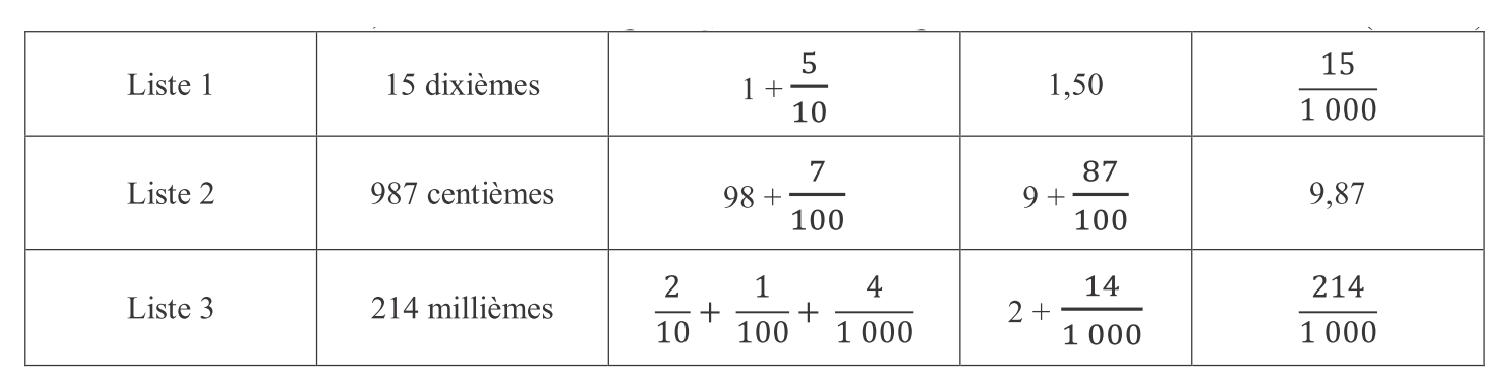
\includegraphics[scale=0.65]{controle1.eps} \\
\end{flushleft}

\exo{5.5}
\includegraphics[scale=0.4]{trefle.eps} Compléter le tableau ci-dessous :

\begin{center}
\includegraphics[scale=1.2]{controle4.eps} 
\end{center}

\newpage

\vspace*{0.1cm}

\exo{1.5} 
\includegraphics[scale=0.4]{trefle.eps} Compléter avec les symboles $\in$ ou $\notin$ : 

\bmul{2}

\bmul{2}

E . . . [CB)\\

A . . . [BF]\\


B . . . [CE)\\


\columnbreak

B . . . (AF)\\

A . . . [BF)\\

C . . . [BE]\\


\emul




\columnbreak

\includegraphics[scale=0.6]{controle2.eps}\\


\emul

\exo{3} 
\includegraphics[scale=0.4]{trefle.eps}  Compléter la figure en ajoutant les noms de chacun des six points  nommés dans les indications suivantes : 

\bmul{2}



- $A \in (d_{1})$ et $A \in (d_{2})$ \hspace*{0.5cm} - $B \in (d_{1})$ et $C \in (d_{1})$\\

- $C \in [AB]$ \hspace*{2.5cm}- $F \notin (d_{1})$ et $F \notin (d_{2})$\\

- $D \in (d_{2})$ et $E \in (d_{2})$ \hspace*{0.5cm}- $D \in [AE)$ et $D \notin [AE]$\\












\columnbreak

\begin{flushright}
\includegraphics[scale=0.6]{controle3.eps}

\end{flushright}
\emul


\exo{3} 
\includegraphics[scale=0.4]{trefle.eps}

\includegraphics[scale=0.8]{demidroite.eps} 


\initq \q Donner les abscisses des points A, B et C : \reponse[1]\\


\q Placer (à l'aide d'une croix bleue) les points E, F et G sur la demi-droite graduée :

\begin{center}
 E(2)  ;  F(5,6)   et   G(quatre-vingts centièmes)
\end{center}





\exo{2}

Avec la règle plate et l'équerre, construire soigneusement sur votre copie double :\\

\bi

\item Tracer une droite (AL)

\item Placer un point $M \in (AC)$ et un point $B \notin (AC)$

\item Tracer la droite $ (d_{1})$ perpendiculaire à la droite (AL) passant par le point M
 
\item Tracer la droite $ (d_{2})$ parallèle à la droite (AM) passant par le point B.\\

\ei



\exo{1.5} Luc doit construire la figure ci-contre. Voici les différentes instructions dans le désordre. \\
\textbf{Réécrire sur votre copie double} les instructions dans le bon ordre.\\



\begin{center}
\includegraphics[scale=0.9]{programmeconstruction.eps} 
\end{center}


\bi	
\item Tracer la droite perpendiculaire à (MU) passant par I. Elle coupe (MU) en O.
\item Tracer la droite perpendiculaire à (MA) passant par U. Elle coupe (MA) en I.
\item Les droites (OH) et (IU) sont sécantes en B.
\item Tracer un triangle MAU.
\item Tracer la droite parallèle à (MA) passant par O. Elle coupe (AU) en H.\\
\ei


\end{document}
